\documentclass[pdflatex,compress,mathserif]{beamer}

%\usetheme[dark,framenumber,totalframenumber]{ElektroITK}
\usetheme[darktitle,framenumber,totalframenumber]{ElektroITK}

\usepackage[utf8]{inputenc}
\usepackage[T1]{fontenc}
\usepackage{lmodern}
\usepackage[bahasai]{babel}
\usepackage{amsmath}
\usepackage{amsfonts}
\usepackage{amssymb}
\usepackage{graphicx}
\usepackage{multicol}

\newcommand*{\Scale}[2][4]{\scalebox{#1}{$#2$}}%

\title{PEMODELAN JARINGAN KOMUNIKASI}
\subtitle{Dynamic Routing Protocols}

\author{Tim Dosen Pengampu}

\begin{document}

\maketitle

\section{Dynamic Routing Protocols vs Static Routes}

\begin{frame}
	\frametitle{Dynamic Routing Protocols}
	\begin{itemize}
		\item When a routing protocol is used, routers automatically advertise their
 best paths to known networks to each other.
		\item Routers use this information to determine their own best path to the
 known destinations.
		\item When the state of the network changes, such as a link going down or a
 new subnet being added, the routers update each other.
		\item Routers will automatically calculate a new best path and update the
 routing table if the network changes.
	\end{itemize}
\end{frame}

\begin{frame}{Dynamic Routing Protocols}
	\begin{itemize}
		\item You can get to these networks via me:
	\end{itemize}
	\begin{center}
		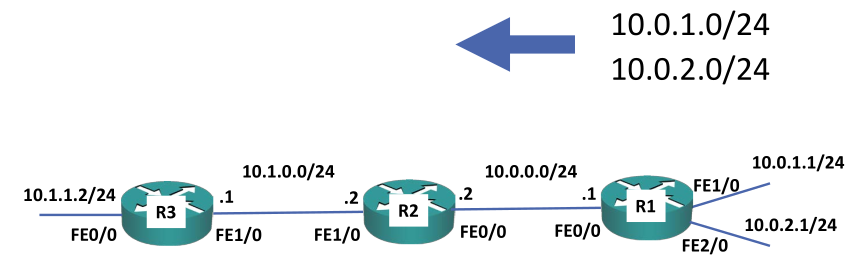
\includegraphics[width=\linewidth]{img/img01}
	\end{center}
\end{frame}

\begin{frame}{Dynamic Routing Protocols}
	\begin{itemize}
		\item Routing Table:
	\end{itemize}
	\begin{center}
		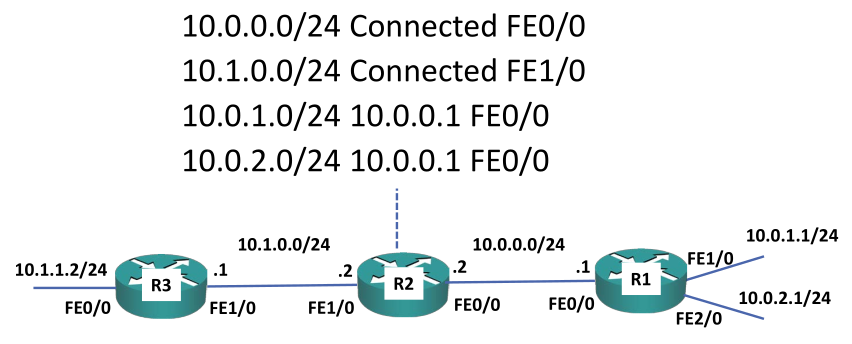
\includegraphics[width=\linewidth]{img/img02}
	\end{center}
\end{frame}

\begin{frame}{Dynamic Routing Protocols}
	\begin{itemize}
		\item You can get to these networks via me:
	\end{itemize}
	\begin{center}
		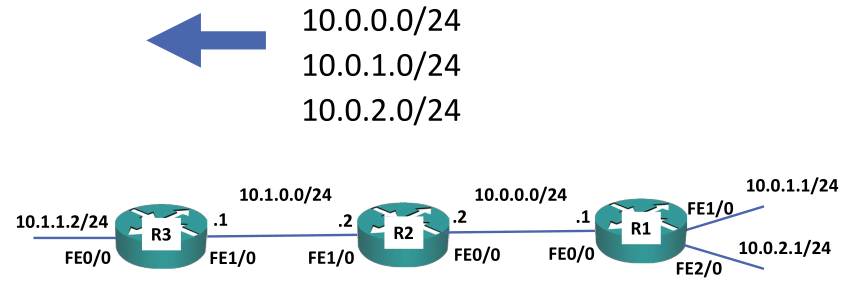
\includegraphics[width=\linewidth]{img/img03}
	\end{center}
\end{frame}

\begin{frame}{Dynamic Routing Protocols}
	\begin{itemize}
		\item Routing Table:
	\end{itemize}
	\begin{center}
		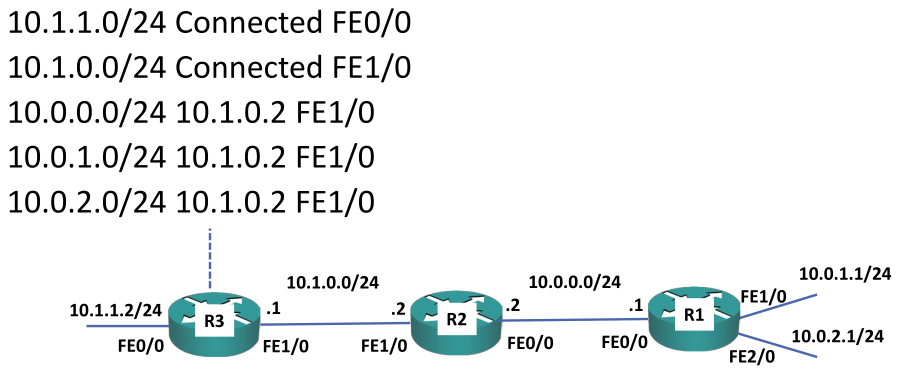
\includegraphics[width=\linewidth]{img/img04}
	\end{center}
\end{frame}

\begin{frame}
	\frametitle{Summary Routes}
	\begin{itemize}
		\item You can get to these networks via me:
	\end{itemize}
	\begin{center}
		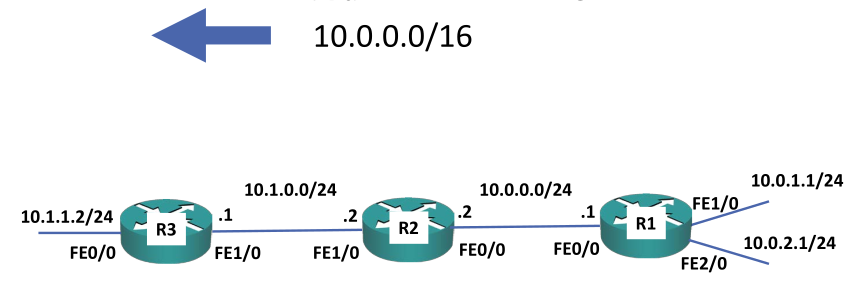
\includegraphics[width=\linewidth]{img/img05}
	\end{center}
\end{frame}

\begin{frame}{Summary Routes}
	\begin{itemize}
		\item Summary routes lead to less memory usage in routers as their routing tables contain less routes
		\item They also lead to less CPU usage as changes in the network only affect
other routers in the same area
		\item For example, if the link on R1 to the 10.0.1.1/24 network goes down, R2
will lose its route there and try to compute a new path
		\item R3 will not be affected as its summary route to 10.0.0.0/16 is unchanged
	\end{itemize}
\end{frame}

\begin{frame}
	\frametitle{Dynamic Routing Protocols\\vs Static Routes}
	\begin{itemize}
		\item Routing protocols are more scalable than administrator defined static
routes.
		\item Using purely static routes is only feasible in very small environments.
	\end{itemize}
\end{frame}

\begin{frame}
	\frametitle{Dynamic Routing Protocol\\Advantages}
	\begin{itemize}
		\item The routers automatically advertise available subnets to each other
without the administrator having to manually enter every route on every
		router.
		\item If a subnet is added or removed the routers will automatically discover
that and update their routing tables.
		\item If the best path to a subnet goes down routers automatically discover
that and will calculate a new best path if one is available.
	\end{itemize}
\end{frame}

\begin{frame}
	\frametitle{Dynamic Routing Protocols\\vs Static Routes}
	\begin{itemize}
		\item Using a combination of a dynamic routing protocol and static routes is
very common in real world environments.
		\item In this case the routing protocol will be used to carry the bulk of the
network information.
		\item Static routes can also be used on an as needed basis. For example for
backup purposes or for a static route to the Internet (which will typically
be injected into the dynamic routing protocol and advertised to the rest
of the routers.)
	\end{itemize}
\end{frame}

\begin{frame}
	\frametitle{Lab}
	\begin{center}
		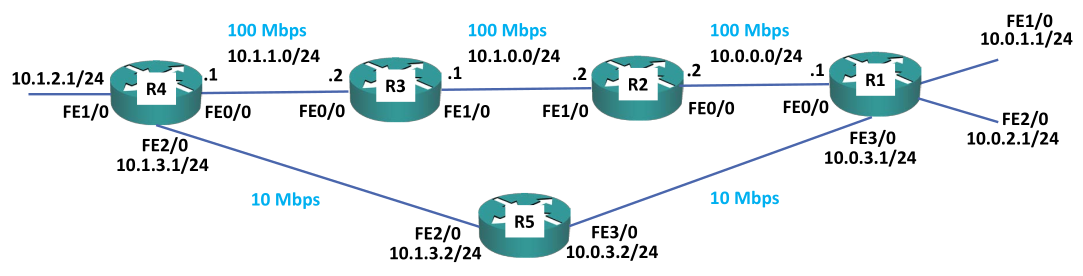
\includegraphics[width=\linewidth]{img/img06}
	\end{center}
\end{frame}

\section{Routing Protocol Types}

\begin{frame}
	\frametitle{Routing Protocol Types}
	\begin{itemize}
		\item Routing protocols can be split into two main types:
		\begin{enumerate}
			\item Interior gateway protocols (IGPs)
			\item Exterior gateway protocols (EGPs)
		\end{enumerate}
		\item Interior gateway protocols are used for routing within an organisation
		\item Exterior gateway protocols are used for routing between organisations
over the Internet
		\item The only EGP in use today is BGP (Border Gateway Protocol)
	\end{itemize}
\end{frame}

\begin{frame}
	\frametitle{Interior Gateway Protocols}
	\begin{itemize}
		\item Interior gateway protocols can be split into two main types:
		\begin{enumerate}
			\item Distance Vector routing protocols
			\item Link State routing protocols
		\end{enumerate}
	\end{itemize}
\end{frame}

\begin{frame}
	\frametitle{Distance Vector Routing Protocols}
	\begin{itemize}
		\item In Distance Vector protocols, each router sends its directly connected
neighbours a list of all its known networks along with its own distance to
each of those networks
		\item Distance vector routing protocols do not advertise the entire network
topology
		\item A router only knows its directly connected neighbours and the lists of
networks those neighbours have advertised. It doesn’t have detailed
topology information beyond its directly connected neighbours
		\item Distance Vector routing protocols are often called 'Routing by rumour'
	\end{itemize}
\end{frame}

\begin{frame}
	\frametitle{Link State Routing Protocols}
	\begin{itemize}
		\item In Link State routing protocols, each router describes itself and its
 interfaces to its directly connected neighbours
		\item This information is passed unchanged from one router to another
		\item Every router learns the full picture of the network including every router,
 its interfaces and what they connect to
	\end{itemize}
\end{frame}

\begin{frame}
	\frametitle{Dynamic Routing Protocols}
	\begin{center}
		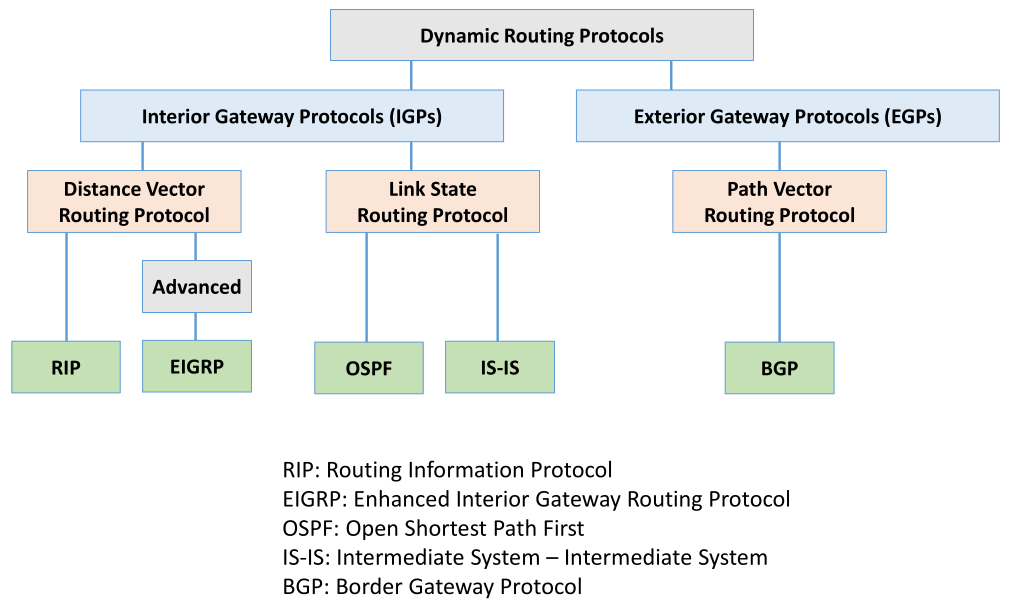
\includegraphics[width=\linewidth]{img/img07}
	\end{center}
\end{frame}

\begin{frame}
	\frametitle{Interior Gateway Protocols}
	\begin{itemize}
		\item All of the IGPs do the same job, which is to advertise routes within an
 organisation and determine the best path or paths
		\item An organisation will typically pick one of the IGPs
		\item If an organisation has multiple IGPs in effect (for example because of a
 merger), information can be redistributed between them. This should
 generally be avoided if possible
	\end{itemize}
\end{frame}

\begin{frame}
	\frametitle{Lab}
	\begin{center}
		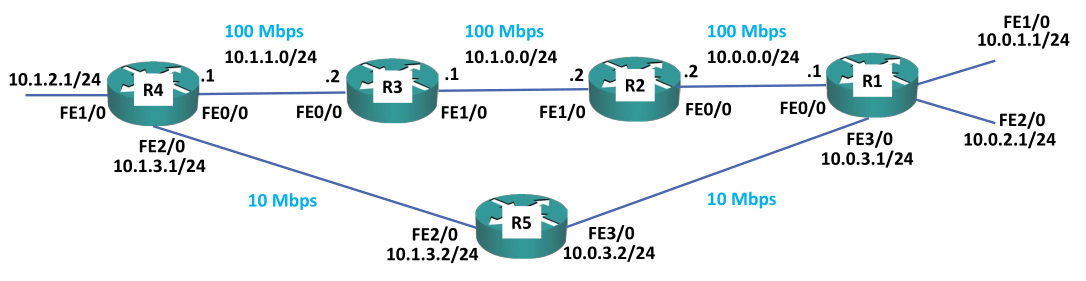
\includegraphics[width=\linewidth]{img/img08}
	\end{center}
\end{frame}

\section{Routing Protocol Metrics}

\begin{frame}
	\frametitle{Metric}
	\begin{itemize}
		\item A router may receive multiple possible paths to get to a destination
network
		\item Only the best path will make it into the routing table and be used
		\item The different IGPs use different methods to calculate the best path to a
destination network
	\end{itemize}
\end{frame}

\begin{frame}{Metric}
	\begin{itemize}
		\item Each possible path will be assigned a ‘metric’ value by the routing
protocol which indicates how preferred the path is
		\item The lowest metric value is preferred
		\item Distance Vector routers advertise to each other the networks they know
about, and their metric to get to each of them
		\item Link State routers advertise all the links in their area of the network to
each other
		\item Each router will take this information and then make an independent
calculation of its own best path to get to each destination
	\end{itemize}
\end{frame}

\begin{frame}{Metric}
	\begin{itemize}
		\item If the best path to a destination is lost (for example because a link went
down) it will be removed from the routing table and replaced with the
next best route
	\end{itemize}
\end{frame}

\begin{frame}
	\frametitle{RIP Metric – Hop Count}
	\begin{itemize}
		\item RIP uses Hop Count as the metric
		\item The maximum hop count by default is 15. Paths which are more than 15
hops away are marked as unreachable
		\item Path R4>5>1 will be preferred for 10.0.1.0/24 in the example below
		\item RIP is typically used only in small or test environments
	\end{itemize}
	\begin{center}
		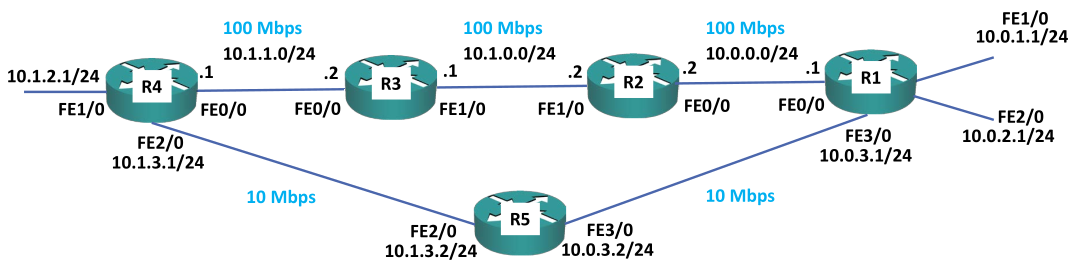
\includegraphics[width=\linewidth]{img/img09}
	\end{center}
\end{frame}

\begin{frame}{RIP Metric – Hop Count}
	\begin{itemize}
		\item RIP uses Hop Count as the metric
	\end{itemize}
	\begin{center}
		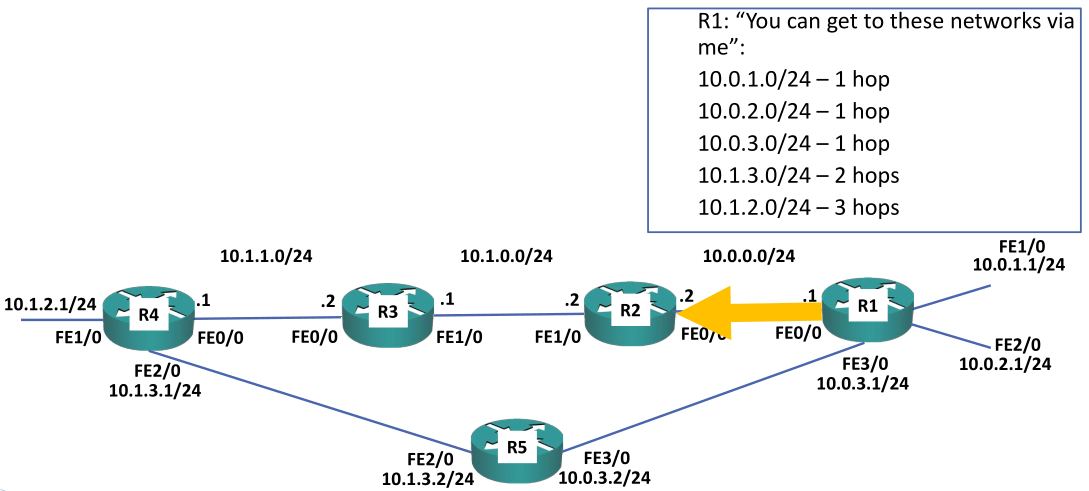
\includegraphics[width=\linewidth]{img/img10}
	\end{center}
\end{frame}

\begin{frame}{RIP Metric – Hop Count}
	\begin{center}
		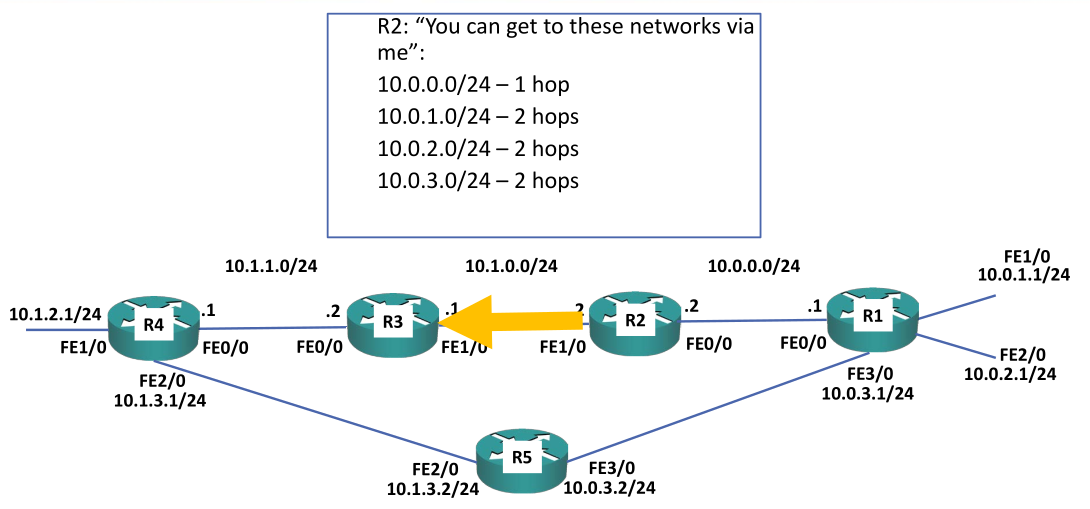
\includegraphics[width=\linewidth]{img/img11}
	\end{center}
\end{frame}

\begin{frame}{RIP Metric – Hop Count}
	\begin{center}
		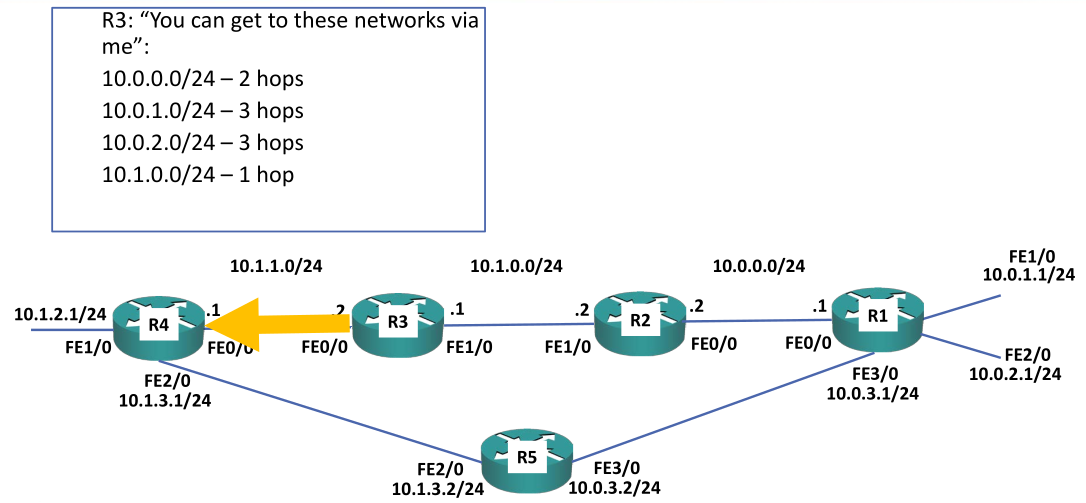
\includegraphics[width=\linewidth]{img/img12}
	\end{center}
\end{frame}

\begin{frame}{RIP Metric – Hop Count}
	\begin{center}
		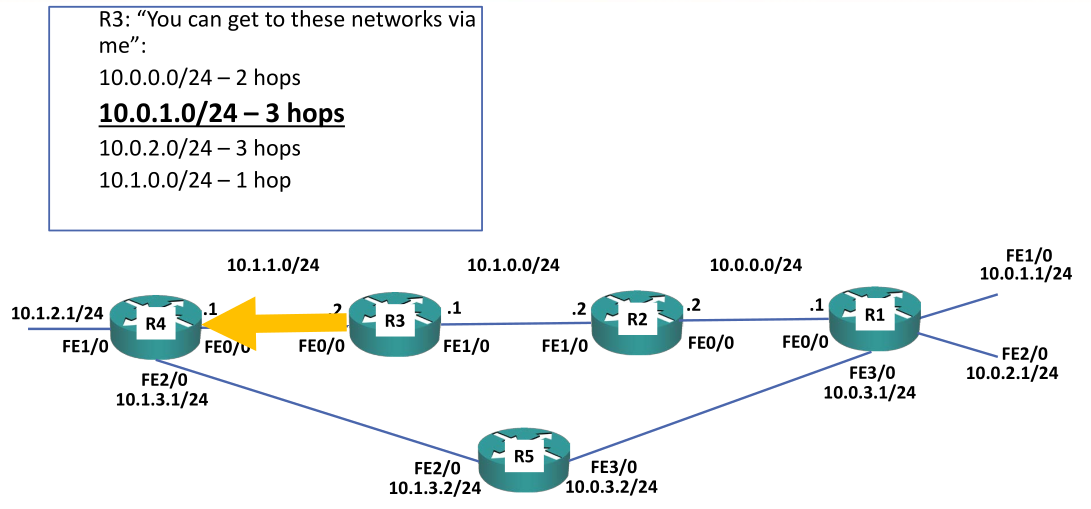
\includegraphics[width=\linewidth]{img/img13}
	\end{center}
\end{frame}

\begin{frame}{RIP Metric – Hop Count}
	\begin{center}
		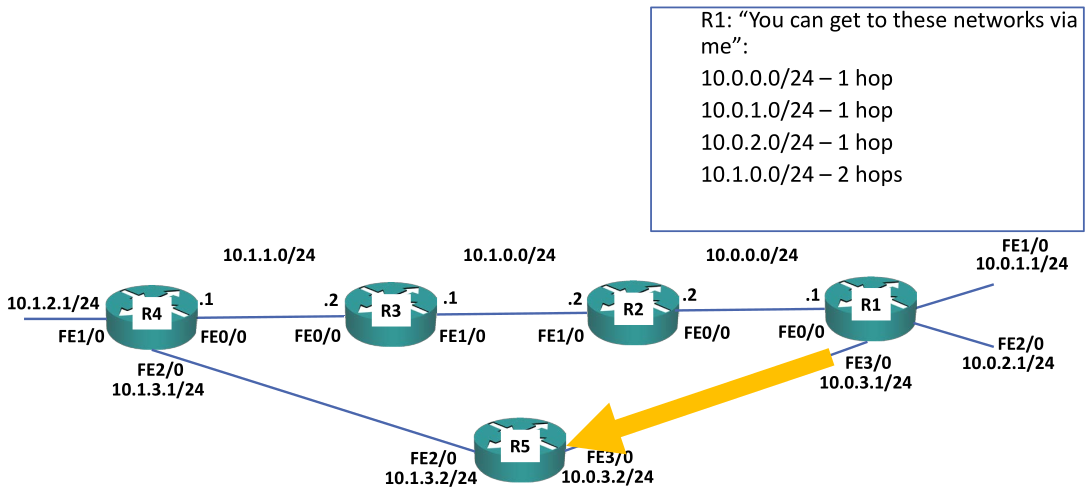
\includegraphics[width=\linewidth]{img/img14}
	\end{center}
\end{frame}

\begin{frame}{RIP Metric – Hop Count}
	\begin{center}
		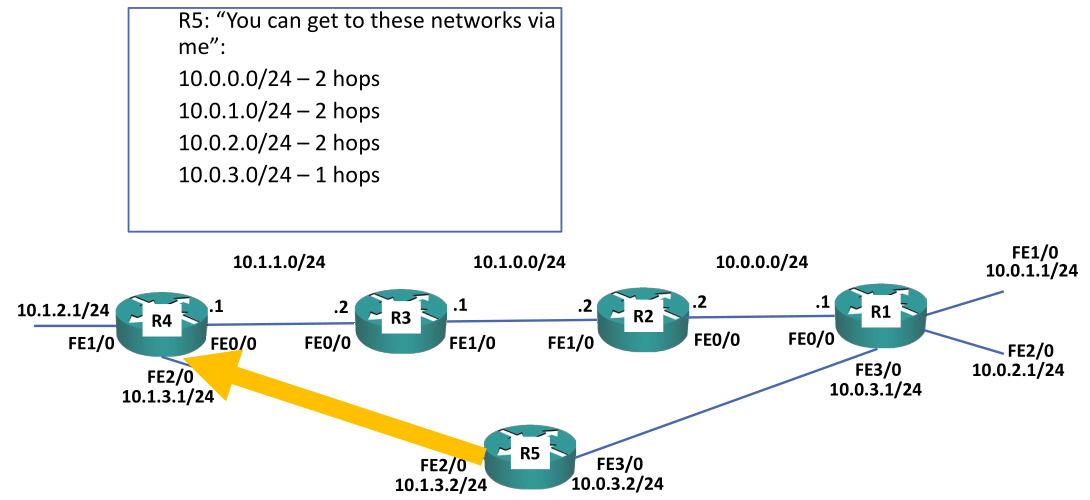
\includegraphics[width=\linewidth]{img/img15}
	\end{center}
\end{frame}

\begin{frame}{RIP Metric – Hop Count}
	\begin{center}
		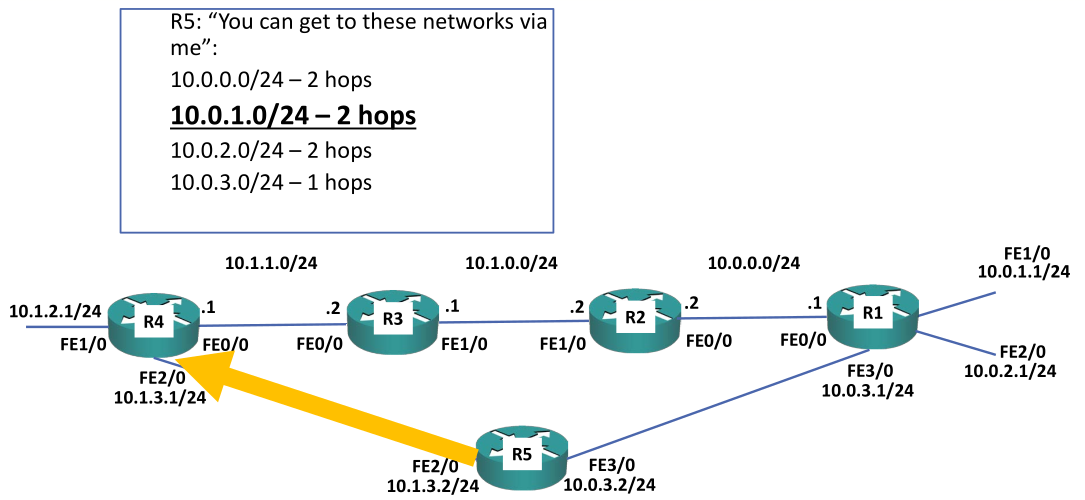
\includegraphics[width=\linewidth]{img/img16}
	\end{center}
\end{frame}

\begin{frame}{RIP Metric – Hop Count}
	R4: I learned 2 possible routes to get to the 10.0.1.0/24 network:
\\
	3 hops via 10.1.1.2 out FE0/0
\\
	2 hops via 10.1.3.2 out F2/0
\\
	I’ll put the best one in my routing table\\
	\begin{center}
		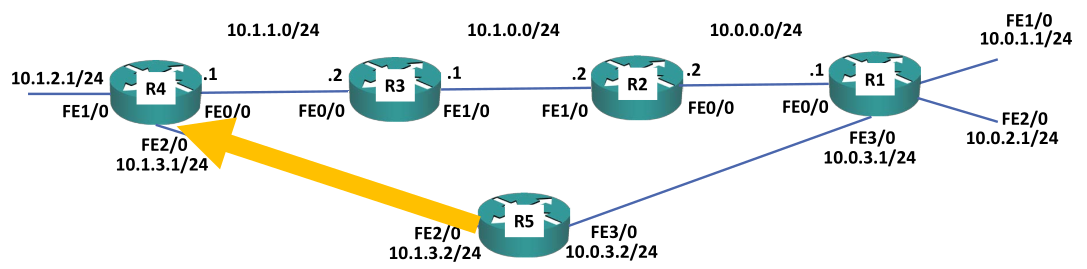
\includegraphics[width=\linewidth]{img/img17}
	\end{center}
\end{frame}

\begin{frame}{RIP Metric – Hop Count}
	\begin{center}
		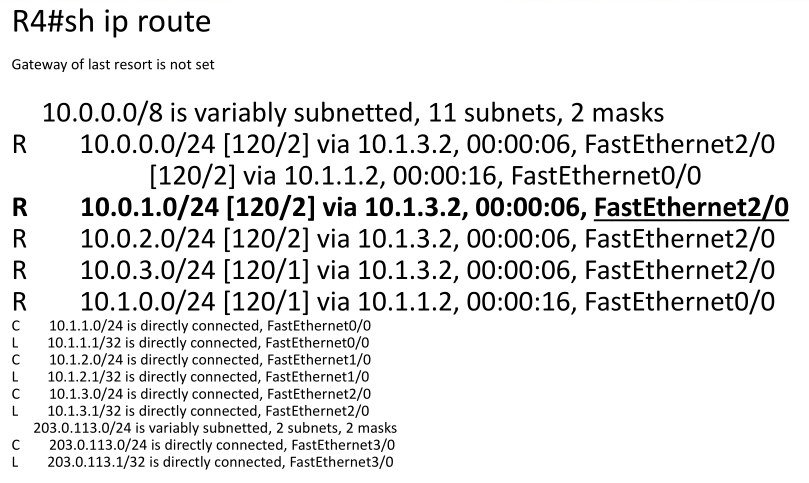
\includegraphics[width=\linewidth]{img/img18}
	\end{center}
\end{frame}

\begin{frame}
	\frametitle{OSPF Metric – Cost}
	\begin{itemize}
		\item OSPF uses ‘Cost’ as the metric, which is automatically derived from
interface bandwidth by default
		\item You can manually configure the cost of links if you want to manipulate
the path
		\item Path R4>3>2>1 will be preferred for 10.0.1.0/24 in the example below
	\end{itemize}
	\begin{center}
		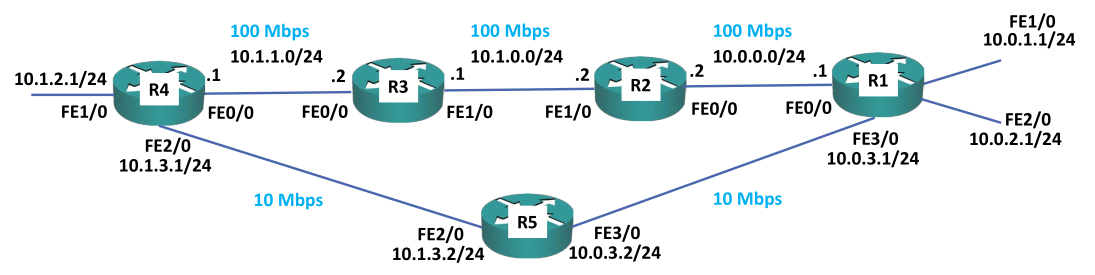
\includegraphics[width=\linewidth]{img/img19}
	\end{center}
\end{frame}

\begin{frame}{OSPF Metric – Cost}
	\begin{center}
		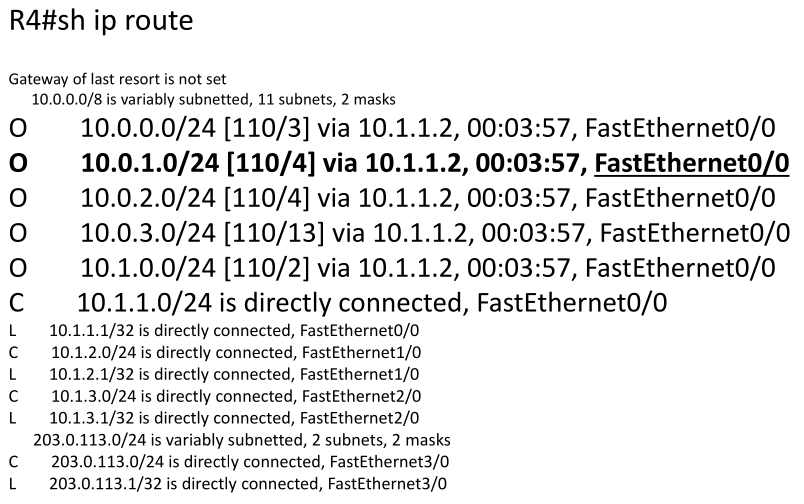
\includegraphics[width=\linewidth]{img/img20}
	\end{center}
\end{frame}

\begin{frame}
	\frametitle{IS-IS Metric – Cost}
	\begin{itemize}
		\item IS-IS also uses 'Cost' as the metric, but it is not automatically derived from interface bandwidth. All links have an equal cost by default
		\item You can manually configure the cost of links if you want to manipulate the path
		\item If you do not manually set the link costs then the path with the lowest hop
count will be used
		\item Path R4>5>1 will be preferred for 10.0.1.0/24 in the example below
	\end{itemize}
\end{frame}

\begin{frame}{IS-IS Metric – Cost}
	\begin{center}
		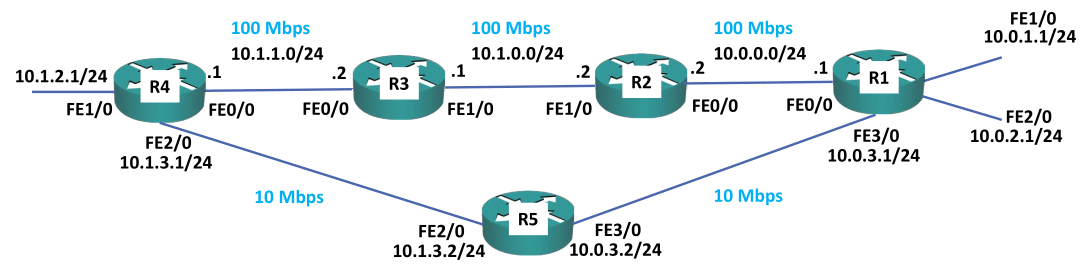
\includegraphics[width=\linewidth]{img/img21}
	\end{center}
\end{frame}

\begin{frame}
	\frametitle{EIGRP Metric}
	\begin{itemize}
		\item EIGRP uses the bandwidth and delay of links to calculate the metric
		\item (Load and reliability can also be considered but are ignored by default)
		\item A fixed delay value is used based on the interface bandwidth, the protocol does
not dynamically measure current delay
		\item You can manually configure the delay on links if you want to manipulate the path
		\item Path R4>3>2>1 will be preferred for 10.0.1.0/24 in the example below
	\end{itemize}
\end{frame}

\begin{frame}{EIGRP Metric}
	\begin{center}
		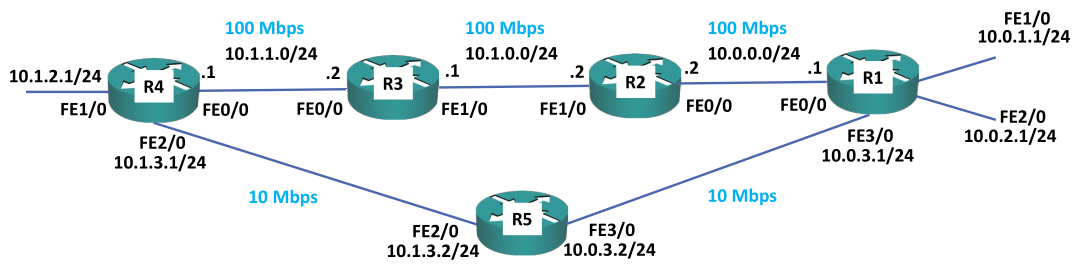
\includegraphics[width=\linewidth]{img/img22}
	\end{center}
\end{frame}

\begin{frame}
	\frametitle{Choosing a Routing Protocol}
	\begin{itemize}
		\item RIP uses hop count and has a default maximum metric of 15. It is not
usually used in production networks because of its scalability limitations.
		\item EIGRP is very simple to maintain, calculates changes very quickly and its
metric calculation will normally choose the best path by default. It is
typically only supported on Cisco routers however.
		\item OSPF’s metric calculation will typically choose the best path by default. It
is an open standard which is supported by all vendor’s routers and is the
most commonly deployed IGP today. It is however more complicated to
maintain than EIGRP.
	\end{itemize}
\end{frame}

\begin{frame}{Choosing a Routing Protocol}
	\begin{itemize}
		\item IS-IS links need to be manually configured or it will use hop count to
determine the best path. It is typically only used in Service Provider
networks or large organisations with their own MPLS network who
choose it because of its scalability.
	\end{itemize}
\end{frame}

\begin{frame}
	\frametitle{Lab}
	\begin{center}
		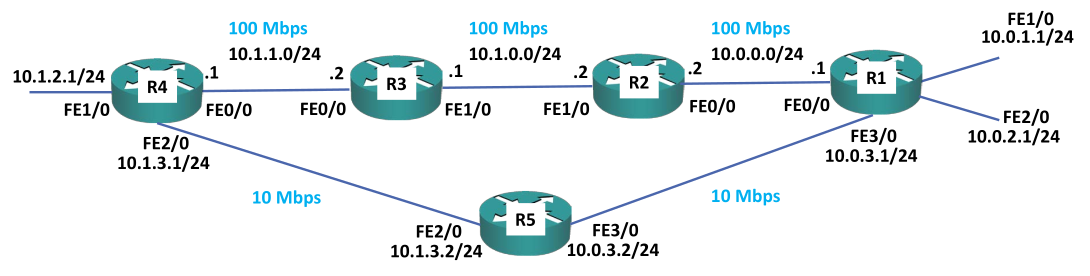
\includegraphics[width=\linewidth]{img/img23}
	\end{center}
\end{frame}

\section{Equal Cost Multi Path}

\begin{frame}
	\frametitle{Equal Cost Multi Path (ECMP)}
	\begin{itemize}
		\item If multiple paths to a destination have an equal metric, the router will
enter all of the paths into the routing table
		\item Equal Cost Multi Path will load balance the outbound traffic to the
destination over the different paths
		\item All IGP routing protocols will perform ECMP by default
		\item EIGRP is the only routing protocol which is capable of UnEqual Cost Multi
Path. It must be manually configured to support this.
	\end{itemize}
\end{frame}

\begin{frame}{Equal Cost Multi Path (ECMP)}
	\begin{itemize}
		\item Both routes to 10.0.1.0/24 will be installed in Router 4’s routing table
		\item Half the traffic will take path R4>3>2>1
		\item Half the traffic will take path R4>5>6>1
	\end{itemize}
	\begin{center}
		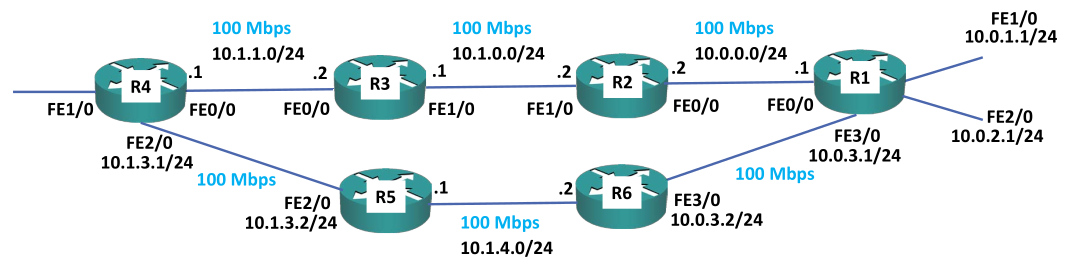
\includegraphics[width=\linewidth]{img/img24}
	\end{center}
\end{frame}

\begin{frame}{Equal Cost Multi Path (ECMP)}
	\begin{itemize}
		\item You can also achieve load balancing with static routes
	\end{itemize}
	\texttt{R4(config)\# ip route 10.0.1.0 255.255.255.0 10.1.1.2
\\
		R4(config)\# ip route 10.0.1.0 255.255.255.0 10.1.3.2}
	\begin{center}
		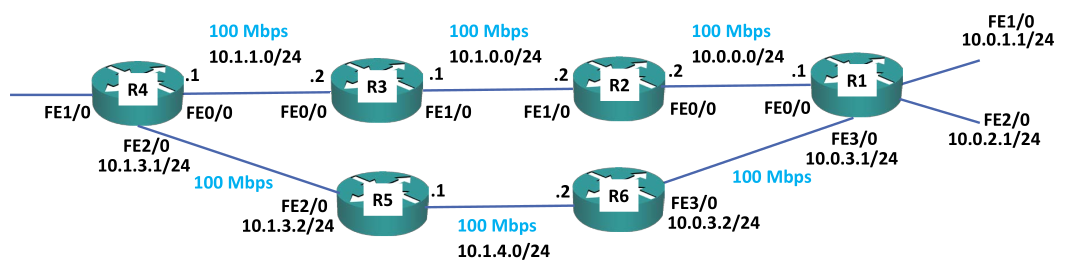
\includegraphics[width=\linewidth]{img/img25}
	\end{center}
\end{frame}

\begin{frame}
	\frametitle{Lab}
	\begin{center}
		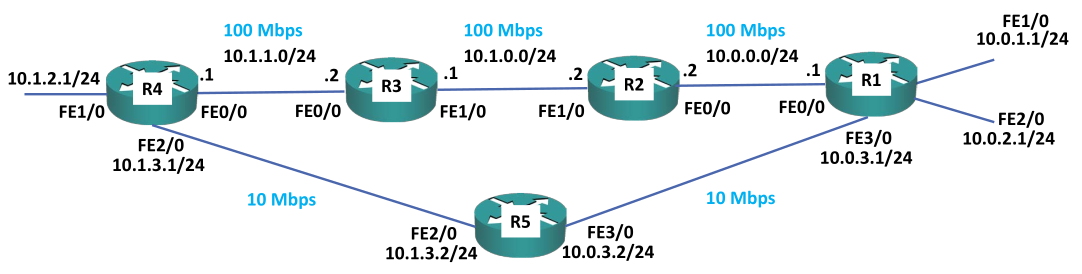
\includegraphics[width=\linewidth]{img/img26}
	\end{center}
\end{frame}

\begin{frame}{Lab}
	\begin{center}
		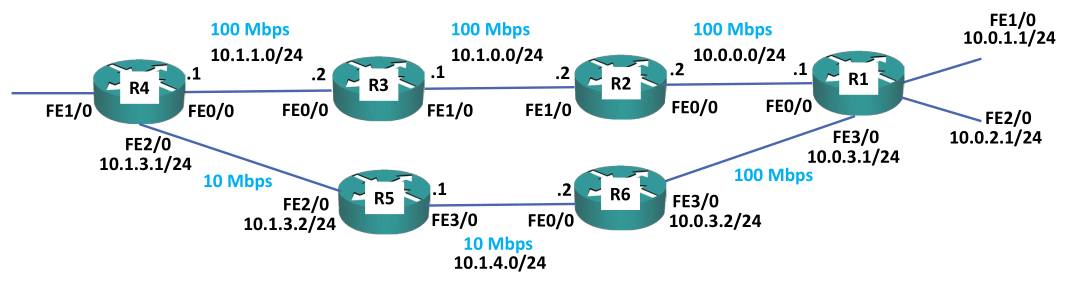
\includegraphics[width=\linewidth]{img/img27}
	\end{center}
\end{frame}

\section{Administrative Distance}

\begin{frame}
	\frametitle{Metric}
	\begin{itemize}
		\item A router will typically only learn routes to a particular destination from a
single routing protocol
		\item When multiple routes to a destination are learned through a routing
protocol, the router will install the path or paths with the best (lowest)
metric into the routing table
		\item Different routing protocols use different methods to calculate the metric
	\end{itemize}
\end{frame}

\begin{frame}{Metric}
	\begin{itemize}
		\item For example in RIP, path A>B>C>D has a hop count of 3, path A>B>D has a
hop count of 2, so A>B>D would be preferred
		\item In OSPF, if path A>B>C>D has a cost of 60, and path A>B>D has a cost of
100, then A>B>C>D would be used
	\end{itemize}
\end{frame}

\begin{frame}
	\frametitle{Administrative Distance}
	\begin{itemize}
		\item If paths to the same destination are received from different routing
protocols, their metrics cannot be compared
		\item For example, a RIP hop count of 5 cannot be compared to an OSPF cost of
60. The comparison would be meaningless because the routing protocols
calculate the metric in completely different ways
		\item The router must use a different method to choose when routes to the
same destination are received from different routing protocols
		\item The Administrative Distance (AD) is used for this
	\end{itemize}
\end{frame}

\begin{frame}{Administrative Distance}
	\begin{itemize}
		\item The Administrative Distance is a measure of how trusted the routing
protocol is
		\item If routes to the same destination are received via different routing
protocols, the protocol with the best (lowest) AD wins
	\end{itemize}
\end{frame}

\begin{frame}
	\frametitle{Default Administrative Distance}
	\begin{center}
		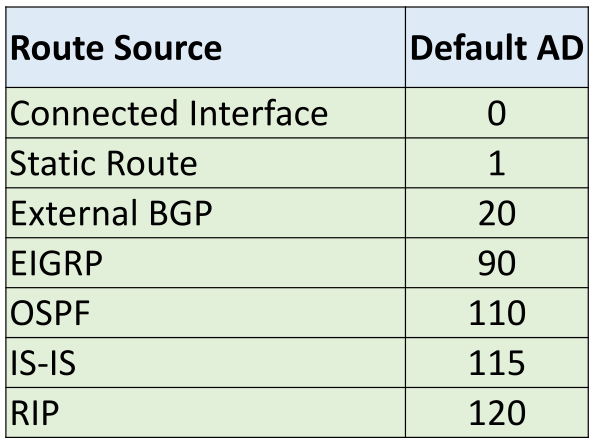
\includegraphics[width=0.7\linewidth]{img/img28}
	\end{center}
\end{frame}

\begin{frame}
	\frametitle{Administrative Distance and Metric}
	\begin{itemize}
		\item Administrative Distance is used to choose between multiple paths
learned via different routing protocols
		\item Metric is used to choose between multiple paths learned via the same
protocol
		\item The Administrative Distance is considered first to narrow the choice
down to the single best routing protocol
		\item The Metric is then considered to choose the best path or paths which
make it into the routing table
	\end{itemize}
\end{frame}

\begin{frame}
	\frametitle{Show ip route}
	\begin{center}
		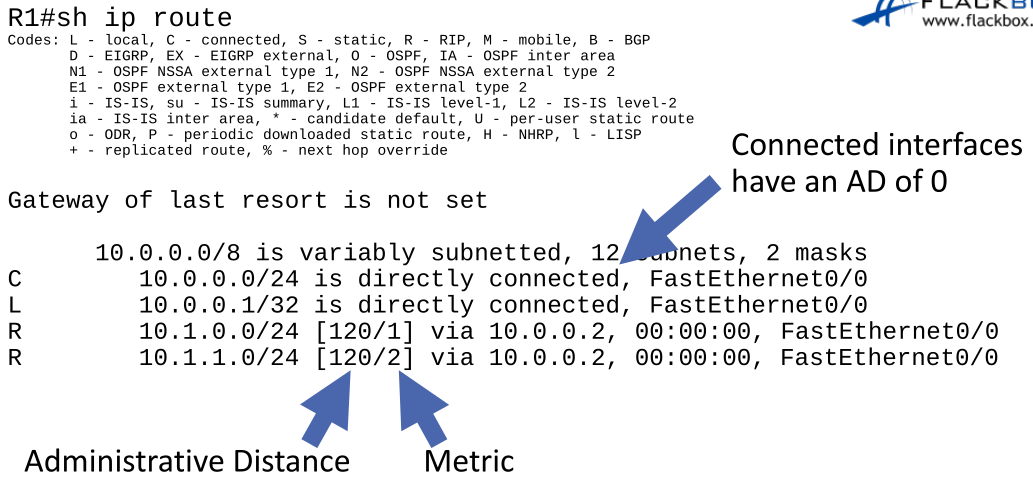
\includegraphics[width=\linewidth]{img/img29}
	\end{center}
\end{frame}

\begin{frame}
	\frametitle{Administrative Distance Example}
	\begin{itemize}
		\item Example: A router receives multiple routes to the 10.10.10.0/24 network
from both OSPF and RIP
		\item When paths to the same destination are received from multiple routing
protocols, the Administrative Distance is considered first
		\item OSPF has a better AD than RIP so the RIP routes will be discarded
	\end{itemize}
\end{frame}

\begin{frame}{Administrative Distance Example}
	\begin{itemize}
		\item The router will then compare the routes received via OSPF and install the
one with the lowest cost in the routing table
		\item If multiple equal cost paths are received via OSPF they will all be installed
in the routing table and the router will load balance outbound traffic to
the destination between them
	\end{itemize}
\end{frame}

\begin{frame}
	\frametitle{Floating Static Routes}
	\begin{itemize}
		\item If the best path to a destination is lost (for example because a link went
down) it will be removed from the routing table and replaced with the
next best route
		\item We might want to configure a static route as a backup for the route
learned via a routing protocol
		\item A problem is that static routes have a default Administrative Distance of 1
which will always be preferred over routes learned via an IGP
	\end{itemize}
\end{frame}

\begin{frame}
	\frametitle{Floating Static Routes – OSPF}
	\begin{itemize}
		\item We can change the Administrative Distance of a static route to make it
act as the backup (rather than the preferred) route
		\item Floating static route for OSPF example
	\end{itemize}
	\begin{center}
		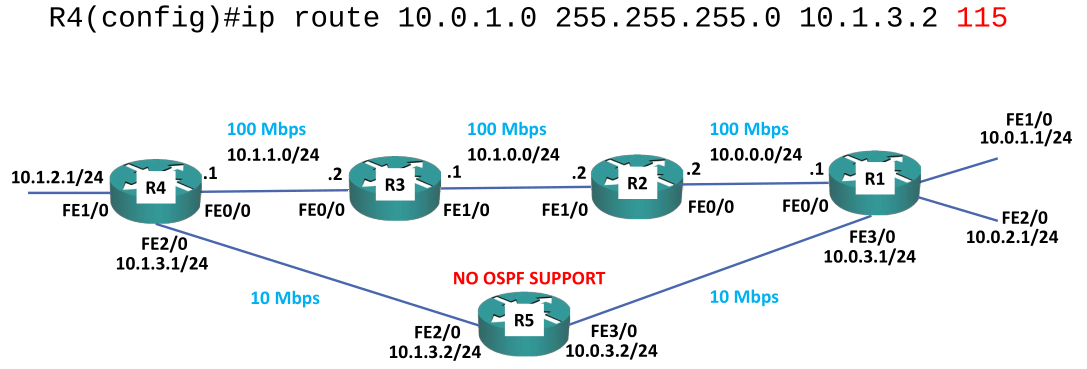
\includegraphics[width=\linewidth]{img/img30}
	\end{center}
\end{frame}

\begin{frame}
	\frametitle{Floating Static Routes – Static Routes}
	\begin{itemize}
		\item Floating static routes can also be used where we are using purely static
routing
	\end{itemize}
	\begin{center}
		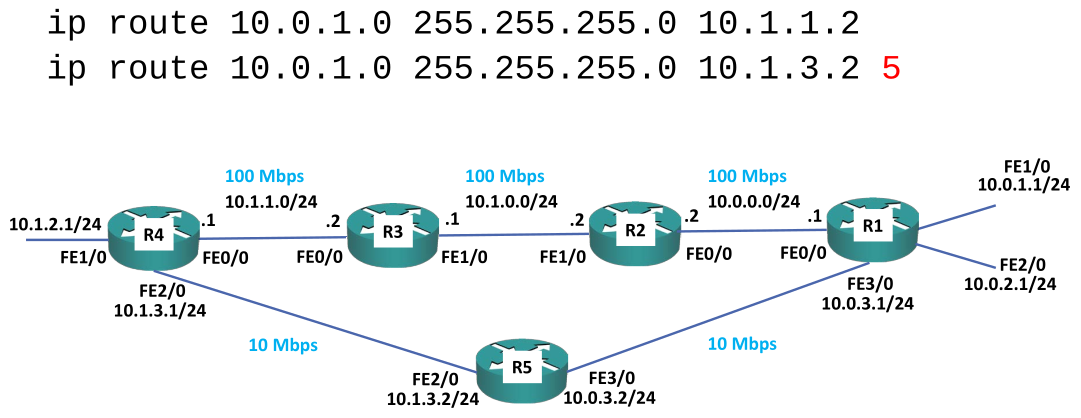
\includegraphics[width=\linewidth]{img/img31}
	\end{center}
\end{frame}

\begin{frame}
	\frametitle{Lab}
	\begin{center}
		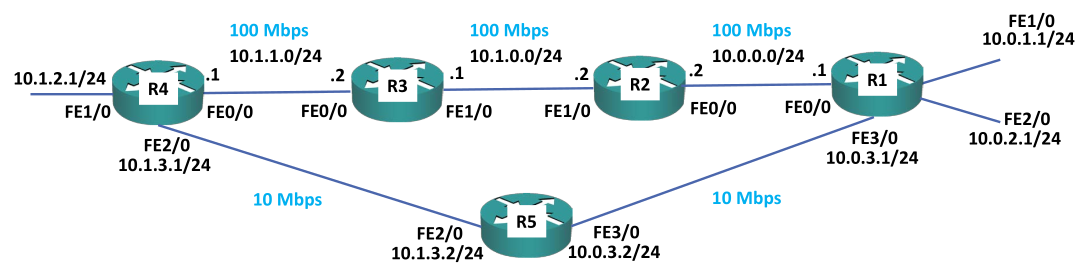
\includegraphics[width=\linewidth]{img/img32}
	\end{center}
\end{frame}

\section{Loopback Interfaces}

\begin{frame}
	\frametitle{Loopback Interfaces}
	\begin{itemize}
		\item Loopback interfaces are logical interfaces
		\item They allow you to assign an IP address to a router or L3 switch, which is
not tied to a physical interface
		\item Because they don’t have any physical attributes which can fail, loopback
interfaces never go down
		\item Loopbacks are logical so they cannot be physically in the same subnet as
other devices, so they are usually assigned a /32 subnet mask to avoid
wasting IP addresses
	\end{itemize}
\end{frame}

\begin{frame}
	\frametitle{Loopback Interface Uses}
	\begin{itemize}
		\item It is best practice to assign a loopback interface to your routers
		\item The loopback is commonly used for traffic that terminates on the router
itself
		\item This could be management traffic, Voice over IP, BGP peering etc.
		\item This provides redundancy if there are multiple paths to the router
		\item The loopback is also used to identify the router (Router ID) in OSPF
	\end{itemize}
\end{frame}

\begin{frame}{Loopback Interface Uses}
	\begin{itemize}
		\item The same loopback interface is usually used for multiple tasks (for
example management and BGP)
		\item Multiple loopbacks can be configured. This is not common and only
usually done where another, separate loopback is required for a special
use case
	\end{itemize}
\end{frame}

\begin{frame}
	\frametitle{Loopback Interfaces}
	\begin{itemize}
		\item For example, my PC is on the 10.1.2.0 subnet and I want to connect to R1
to manage it
		\item If the top path goes down, I cannot connect to 10.0.0.1
		\item If the bottom path goes down, I cannot connect to 10.0.3.1
	\end{itemize}
	\begin{center}
		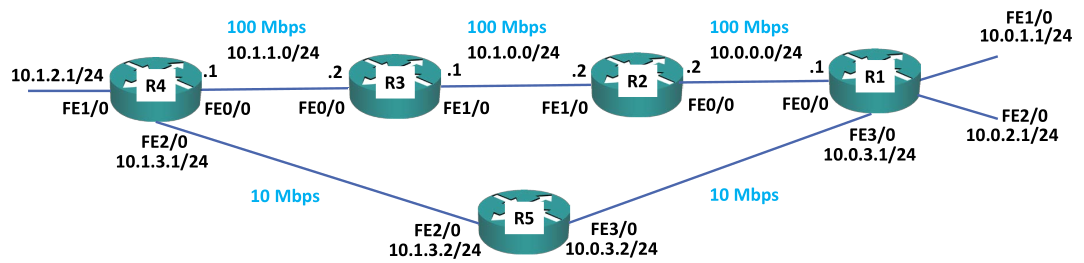
\includegraphics[width=\linewidth]{img/img33}
	\end{center}
\end{frame}

\begin{frame}
	\frametitle{Loopback Interfaces}
	\begin{itemize}
		\item I add interface Loopback 0 with the IP address 192.168.1.1/32
		\item I advertise 192.168.1.1/32 in my routing protocol
		\item R4 learns the two paths to 192.168.1.1
		\item I can still connect to 192.168.1.1 even if either path goes down
	\end{itemize}
	\begin{center}
		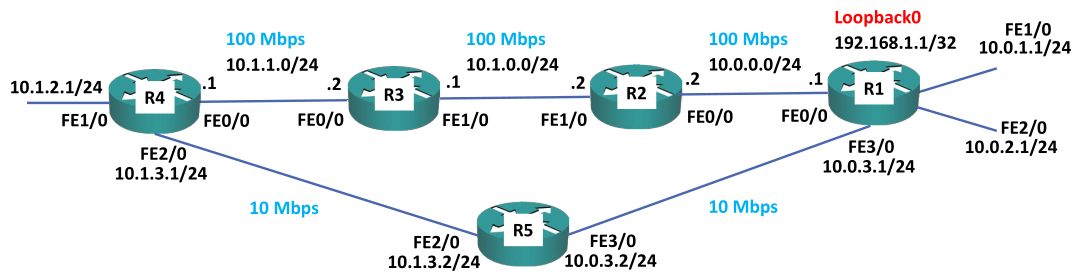
\includegraphics[width=\linewidth]{img/img34}
	\end{center}
\end{frame}

\begin{frame}
	\frametitle{Lab}
	\begin{center}
		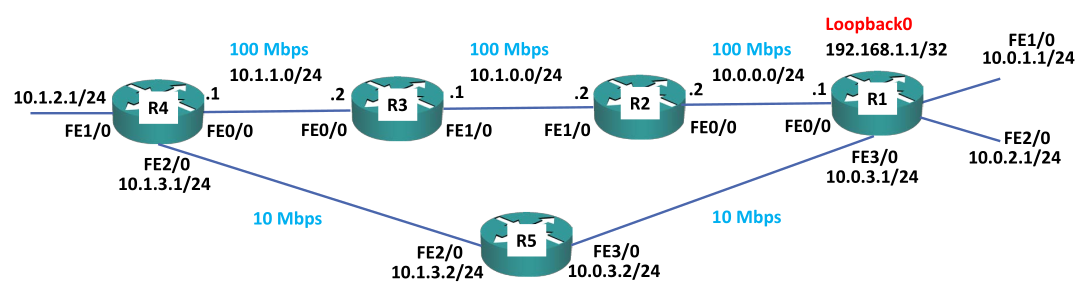
\includegraphics[width=\linewidth]{img/img35}
	\end{center}
\end{frame}

\section{Adjacencies and Passive Interfaces}

\begin{frame}
	\frametitle{Adjacencies}
	\begin{itemize}
		\item IGP routing protocols are configured under global configuration mode
and then enabled on individual interfaces
		\item When the routing protocol is enabled on an interface the router will look
for other devices on the link which are also running the routing protocol
		\item The router does this by sending out and listening for hello packets
		\item When a matching peer is found, the routers will form an adjacency with
each other
		\item They will then exchange routing information
	\end{itemize}
\end{frame}

\begin{frame}{Adjacencies}
	\begin{itemize}
		\item Modern routing protocols use multicast for the hello packets
		\item This is more efficient than broadcast which was used by earlier protocols
		\item Only routers which are running the same routing protocol will process
the packet
	\end{itemize}
\end{frame}

\begin{frame}
	\frametitle{Adjacency Example}
	\begin{itemize}
		\item The IP subnets configured on the interfaces which are enabled for the
routing protocol will be included in its updates
		\item For example, R1 has a routing protocol enabled on the Loopback0
interface and FastEthernet0/0 and 1/0
		\item The routing protocol is not enabled on FastEthernet2/0
		\item RC belongs to a partner organisation we do not want to send internal
network information to
	\end{itemize}
	\begin{center}
		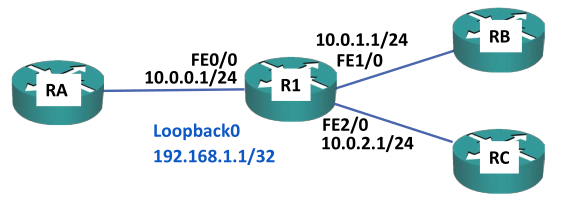
\includegraphics[width=0.6\linewidth]{img/img36}
	\end{center}
\end{frame}

\begin{frame}{Adjacency Example}
	\begin{itemize}
		\item R1 will send out and listen for hello packets on the Loopback0 interface
and FastEthernet0/0 and 1/0
		\item It will form adjacencies with any routers running the same protocol on
those links – RA and RB
		\item It will not send out or listen for hello packets on FastEthernet2/0
		\item It will not form an adjacency with RC
		\item (We will use static routes for the extranet traffic with RC)
	\end{itemize}
	\begin{center}
		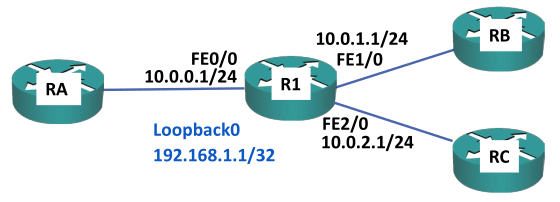
\includegraphics[width=0.6\linewidth]{img/img37}
	\end{center}
\end{frame}

\begin{frame}{Adjacency Example}
	\begin{itemize}
		\item R1 will advertise IP subnets to RA and RB:
\\
		10.0.0.0/24
\\
		10.0.1.0/24
\\
		192.168.1.1/32
		\item It will not advertise 10.0.2.0/24
		\item RA and RB will not learn routes to 10.0.2.0/24
	\end{itemize}
	\begin{center}
		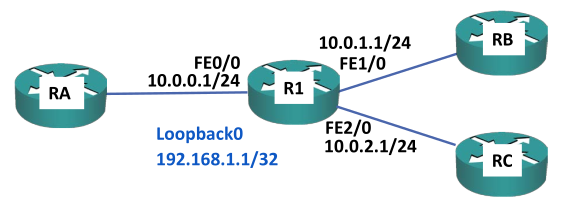
\includegraphics[width=0.6\linewidth]{img/img38}
	\end{center}
\end{frame}

\begin{frame}
	\frametitle{Passive Interfaces}
	\begin{itemize}
		\item Passive interfaces allow you to include an IP subnet in the routing
protocol without sending updates out of the interface
		\item If FastEthernet2/0 is configured as a passive interface, RA and RB will
learn routes to 10.0.2.0, but internal network information will not be
sent to RC
	\end{itemize}
	\begin{center}
		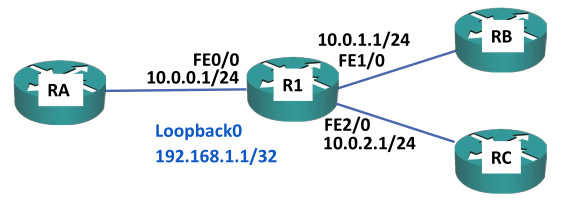
\includegraphics[width=0.6\linewidth]{img/img39}
	\end{center}
\end{frame}

\begin{frame}{Passive Interfaces}
	\begin{itemize}
		\item It is best practice to configure loopback interfaces as passive interfaces
		\item It is impossible to form an adjacency on a loopback interface because
they are not physical interfaces
		\item Making the loopback passive means that it will be advertised by the
routing protocol but it will not waste resources sending out and listening
for hello packets
	\end{itemize}
	\begin{center}
		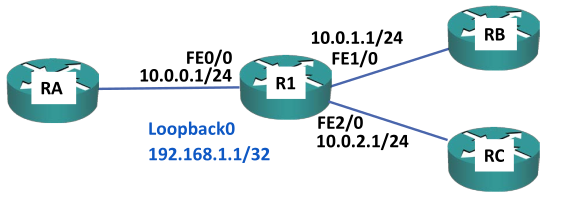
\includegraphics[width=0.6\linewidth]{img/img40}
	\end{center}
\end{frame}

\begin{frame}{Passive Interfaces}
	\begin{itemize}
		\item Passive interfaces are used on:
		\begin{itemize}
			\item Loopback interfaces
			\item Physical interfaces where the device on the other side belongs to
another organisation. We do not want to send routing information
out but we do want our internal devices to know about the link
		\end{itemize}
	\end{itemize}
\end{frame}

\begin{frame}
	\frametitle{Lab}
	\begin{center}
		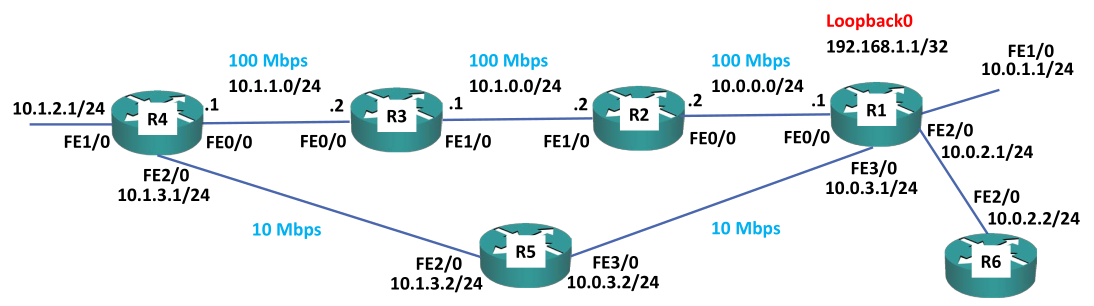
\includegraphics[width=\linewidth]{img/img41}
	\end{center}
\end{frame}

\end{document}
